\documentclass{memoir}
%
% some macro packages
%
\usepackage[utf8]{inputenc}    % smart input of funny chars
\usepackage[T1]{fontenc}       % also for the font encoding
\usepackage{longtable}         % tables longer than one page
\usepackage{calc}
\usepackage{exscale}           % large summation signs in 11pt
\usepackage{array}             % nice tables
\usepackage{subcaption} %For subfigures
\usepackage{wrapfig} % for wrapping text around figures
\usepackage{xspace}            % better spacing after macros
\usepackage{stackengine} 	%for stacking text in diagrams
\setstackEOL{\\}
\usepackage{ifdraft}           % to determine whether draft mode
\usepackage{xparse} %for macros with more than one optional argument
\usepackage{imakeidx} %for index
\usepackage{appendix}
\usepackage[symbols, record]{glossaries-extra}
\usepackage[expansion=false    % no font expansion
           ]{microtype}        % only protrusion
\usepackage[backend = biber,
backref = true,
style = alphabetic,
maxcitenames = 99,
maxbibnames = 99,
mincitenames = 5]{biblatex}

\usepackage[
draft,		%no links
final,                    % treat as final
plainpages=false,              % whatever that means
pdfpagelabels=true,            % strange options
pdfencoding=auto,              % getting worse
unicode=true,                  % unicode is always nice
hypertexnames=true,            % needs both to get index *and*
naturalnames=true,              % crossrefs correct
colorlinks,
linkcolor={blue!70!black},
citecolor={blue!50!black},
urlcolor={blue!80!black}
]{hyperref}                    % hyperrefs are cool!



 



%
% Bibliography with BibLaTex
%
%\DeclareNameAlias{default}{last-first}

\addbibresource{phd-thesis.bib}

%
% Index
%
%\makeindex[intoc,options= {-s phd-index.ist}]

 
%
% Text starts here
%



% Macros imported from macros-phd-thesis.tex
\newcommand{\Ann}{\operatorname{Ann}}
% Orbit space functor

\newcommand{\Total}{{\scriptscriptstyle\script{T}}}
% Normalizer

\newcommand{\Wobs}{{\scriptscriptstyle\script{N}}}
% Null

\newcommand{\Null}{{\scriptscriptstyle\script{0}}}
% Total

\newcommand{\TOTAL}{\script{T}}
% Normalizer

\newcommand{\WOBS}{\script{N}}
% Null

\newcommand{\NULL}{\script{0}}
% Index for strong constraint objects

\newcommand{\ConAlg}{{\Con\Algebras}}

\newcommand{\ConMfld}{{\Con\Manifolds}}

\newcommand{\ConCinfty}{\Con\Cinfty}
% Smooth strong constraint functions

\newcommand{\strtensor}[1][{}]{\mathbin{\boxtimes_{\scriptscriptstyle{#1}}}}
% Strong tensor product for embedded things

% Vanishing ideal
\newcommand{\vanishing}{\spacename{I}}
% Poisson Normalizer
\newcommand{\Pnormalizer}{\mathcal{B}}
% Constraint prefix
\newcommand{\Con}{\categoryname{C}}
% Categories of constraint Modules
\newcommand{\ConMod}{\Con\Modules}


%Copy ChairXthesis

\let\footruleskip\undefined
\usepackage{fancyhdr}          % cool headers
\usepackage{xkeyval}           % key-value options
\usepackage[multiuser]{fixme}  % correction notes, warnings etc.
\usepackage{enumitem}
\usepackage{tikz}              % for commutative diagrams and

\usepackage{nchairx} % additional packages

%
% tikz libraries to be loaded, feel free to add more...
%
\usetikzlibrary{cd,arrows,intersections,matrix,calc,fadings,decorations.pathreplacing,positioning,patterns,decorations.markings,decorations.pathmorphing,calc}
\usetikzlibrary[patterns,patterns.meta]

 

 



%
% TikzCD Settings
%
\tikzcdset{
	row sep/normal=2.7em,
	column sep/normal=3.6em}

%
% List environments
%

\newlist{propertieslist}{enumerate}{1}
\setlist[propertieslist, 1]{topsep = 0.2em,
	partopsep = 0em,
	itemsep = 0.2em,
	parsep = 0.1em,
	label=\textit{\alph*.)}}

\newlist{structurelist}{enumerate}{1}
\setlist[structurelist, 1]{topsep = 0.2em,
	partopsep = 0em,
	itemsep = 0.2em,
	parsep = 0.1em,
	label=\textit{\Alph*.)}}

 



\begin{document}



\paragraph{Geometric Reduction}
In classical mechanics symmetry reduction plays an important role.
Mathematically, this is usually phrased in terms of Marsden-Weinstein reduction \cite{marsden.weinstein:1974a} on a symplectic manifold $(M,\omega)$.
For this assume that a connected Lie group $\group{G}$ acts on $M$ in a Hamiltonian fashion, i.e.
there exists a momentum map $J \colon M \to \liealg{g}^*$, with $\liealg{g}$ denoting the Lie algebra of $\group{G}$,
such that
\begin{equation}
	\phi(\xi) = X_{J_\xi}
\end{equation}
for $\xi \in \liealg{g}$, and $\phi$ denoting the infinitesimal action of $\liealg{g}$.
If $0 \in \liealg{g}$ is a value and regular value of $J$, then $C \coloneqq J^{-1}(\{0\})$
is a closed submanifold of $M$.
Moreover, suppose that $\group{G}$ acts freely and properly on $C$, then
\begin{equation}
	M_\red \coloneqq C / \group{G}
\end{equation}
is a symplectic manifold with symplectic form $\omega_\red$ fulfilling $\pi^*\omega_\red = \iota^*\omega$,
with $\iota \colon C \to M$ the inclusion and $\pi \colon C \to M_\red$ the canonical projection.
It turns out that $C$ is a coisotropic submanifold of $M$ and that the above reduction procedure can actually be done for any coisotropic submanifold of a Poisson manifold.
Such coisotropic submanifolds and their reduction were introduced by Weinstein in \cite{weinstein:1988a} based on ideas
of Poisson reduction from \cite{marsden.ratiu:1086a}, see also \cite{stasheff:1997a}.
For this consider a Poisson manifold $(M,\pi)$, with $\argument^\sharp \colon T^*M \to TM$ denoting the corresponding musical homomorphism.
Then a submanifold $C$ of $M$ is coisotropic if and only if 
\begin{equation}
	\Ann(T_pC)^\# \subseteq T_pC
\end{equation}
for all $p \in C$.
Every such coisotropic submanifold carries a so-called characteristic distribution $D \subseteq TC$ spanned by the 
Hamiltonian vector fields $X_f$ for all functions $f$ vanishing on $C$.
\begin{figure}[t]
	\centering
	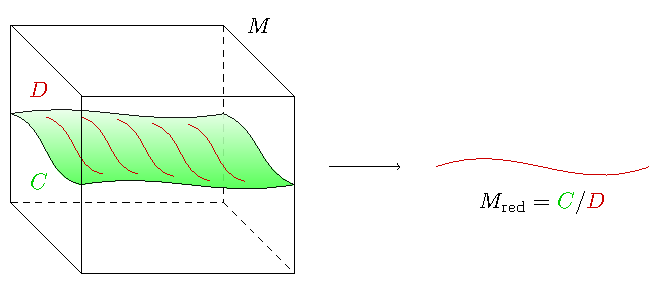
\includegraphics{constraintmanifold-Dippel.pdf}
	\caption{Reduction of coisotropic submanifold $C \subseteq M$ with characteristic distribution $D$.}
	\label{fig:ConstraintManifold}
\end{figure}
In the above case of the Marsden-Weinstein reduction of a symplectic manifold the leaves of this distribution
are given by the orbits of the group action on $C$.
If the characteristic distribution is nice enough, we can construct a reduced manifold
\begin{equation}
	M_\red \coloneqq C / D,
\end{equation}
see \cite[fig:ConstraintManifold]{Dippell2023}, which carries a Poisson structure $\pi_\red$ induced by the Poisson structure $\pi$ on $M$.


\paragraph{Algebraic Reduction}
The general strategy is now to reformulate the geometric situation of a coisotropic submanifold equipped with its characteristic distributions in algebraic terms, similar to the way the algebra of observables $\Cinfty(M)$ is used to algebraically describe the manifold $M$.
Any closed submanifold $C \subseteq M$ can be described in terms of functions by its vanishing ideal
 {vanishingIdeal}
\begin{equation}
	\vanishing_C = \left\{ f \in \Cinfty(M) \bigm| f\at{C} = 0 \right\} \subseteq \Cinfty(M).
\end{equation}
Similarly, the foliation induced by any distribution $D \subseteq TM$ can be encoded by the subalgebra
 {invariantFunctions}
\begin{equation}
	\Cinfty(M)^D = \{ f \in \Cinfty(M) \mid \Lie_X f = 0 \text{ for all } X \in \Secinfty(D) \} \subseteq \Cinfty(M).
\end{equation}
Now for a coisotropic submanifold $C \subseteq (M,\pi)$ the characteristic distribution $D$ is only defined on $C$.
This leads us to consider the subalgebra
 {locallyInvariantFunctions}
\begin{equation}
	\Cinfty_D(M) = \{ f \in \Cinfty(M) \mid \Lie_X f\at{C} = 0 \text{ for all } X \in \Secinfty(D) \} \subseteq \Cinfty(M)
\end{equation}
instead.
Note that the vanishing ideal $\vanishing_C$ is contained in $\Cinfty_D(M)$.
Thus we have established a correspondence
\begin{equation} \label{eq:GeometryAlgebraCorrespondenceConstraint}
	(M,C,D)  \leftrightsquigarrow (\Cinfty(M), \Cinfty_D(M), \vanishing_C)
\end{equation}
between a manifold $M$ equipped with a closed submanifold $C$ on one side and a distribution $D$ on $C$ and
its algebra of functions $\Cinfty(M)$ equipped with the subalgebra $\Cinfty_D(M)$
of functions which are invariant on $C$ and the vanishing ideal $\vanishing_C$ on the other side.
Motivated by coisotropic reduction there is a reduction procedure for both sides of this correspondence.
Namely, on the geometric side, under the assumption of a simple distribution, 
we can construct the reduced manifold $M_\red \coloneqq C / D$ as before, 
while on the algebraic side we can always construct the reduced algebra
\begin{equation}
	\Cinfty(M)_\red = \Cinfty_D(M) / \vanishing_C.
\end{equation}
It is then easy to see that $\Cinfty(M)_\red \simeq \Cinfty(M_\red)$
is just the algebra of functions on the reduced manifold.
If we consider again the setting of a coisotropic submanifold $C \subseteq M$
then one can show that $\vanishing_C$ is a Poisson subalgebra of $(\Cinfty(M), \{\argument, \argument\})$
and that $\Cinfty_D(M)$ coincides with the Poisson normalizer
\begin{equation}
	\Pnormalizer_C = \{ f \in \Cinfty(M) \mid \{f,g\} \in \vanishing_C \text{ for all } g \in \vanishing_C\}	
\end{equation}
of $\vanishing_C$.
In particular, $\vanishing_C$ becomes a Poisson ideal in the Poisson subalgebra $\Pnormalizer_C$, and
therefore $\Cinfty(M)_\red$ carries itself a Poisson bracket, which turns
$M_\red$ into a Poisson manifold.

\paragraph{Constraint Algebras and their Deformations}
We now seek to carry over the basic ideas of deformation quantization to this more structured situation.
This means we want to treat the triple $(\Cinfty(M), \Cinfty_D(M),\vanishing_C)$
as a single algebraic entity and study deformations of it.
Thus we use $(\Cinfty(M), \Cinfty_D(M),\vanishing_C)$ as the motivating example to define an (embedded)
\emph{constraint algebra} $\algebra{A}$ as consisting of a unital associative algebra $\algebra{A}_\Total$
together with a unital subalgebra $\algebra{A}_\Wobs$ and an ideal $\algebra{A}_\Null \subseteq \algebra{A}_\Wobs$.
The subscript $\WOBS$ is supposed to remind the reader of the coisotropic situation, where $\algebra{A}_\Wobs$ is given as 
the Poisson normalizer of the Poisson subalgebra $\algebra{A}_\Null$.

In a next step we can try to define formal deformations of constraint algebras by taking the classical definition of a formal deformation and formally replace algebras by constraint algebras.
In particular, replacing $\Cinfty(M)$ by the constraint algebra $(\Cinfty(M), \Cinfty_D(M), \vanishing_C)$
To make sense of this we first need to clarify some notions:
\begin{cptitem}
	\item What are modules over constraint algebras and their tensor products?
	\item What are constraint multidifferential operators?
	\item Is there a cohomology theory governing the deformation problem of constraint algebras?
\end{cptitem}
We will answer these questions by taking a categorical point of view:
constraint algebras can be realized as monoid objects internal to a certain monoidal category 
$\ConMod_\field{k}$ equipped with a tensor product $\tensor[\field{k}]$, whose objects will be called
constraint $\field{k}$-modules.
By abstract categorical considerations, the definition and some first properties
of constraint modules over constraint algebras, as well as their tensor products, are then fixed.
In contrast to classical categories of modules, the categories of constraint modules will not form abelian categories.
This will lead to effects not present in classical module theory, and forces us to thoroughly examine even the most basic constructions of constraint modules.

This categorical approach will immediately allow us to find constraint analogues of many other classical algebraic concepts, such as derivations, groups, vector spaces, Lie algebras etc.
All these constraint notions will consist of a classical object as $\TOTAL$-component, together with a subobject as
$\WOBS$-component and an equivalence relation or ideal as $\NULL$-component.
Then, by construction, there is always a reduction procedure, defined by taking the quotient of the $\WOBS$-component by the $\NULL$-component, which by definition always yields a classical object.
It should be noted that the motivating example $(\Cinfty(M), \Cinfty_D(M),\vanishing_C)$
has additional properties not accounted for in the definition of constraint algebras, namely that
$\vanishing_C$ is an ideal not only in $\Cinfty_D(M)$ but in all of $\Cinfty(M)$.
Such constraint algebras will be called strong, and their modules will allow for two different canonical tensor products
$\tensor$ and $\strtensor$, whose interplay will be an important piece of study.
Note however that, since we are interested in non-commutative deformations of constraint algebras we should not expect
$\algebra{A}_\Null$ to stay a two-sided ideal in $\algebra{A}_\Total$ after deformation, see Lu's coisotropic creed \cite{lu:1993a}.
Even in the classical geometric situation we will encounter examples of honest non-strong constraint algebras.



\paragraph{Constraint Manifolds and Vector Bundles}
Consider again the correspondence \eqref{eq:GeometryAlgebraCorrespondenceConstraint}.
Here, on the algebraic side, we have a subobject together with an equivalence relation on the subobject which is compatible with the structure of the subobject in a suitable sense.
In our example we have a subalgebra and an ideal inside this subalgebra.
On the geometric side, the triple $(M,C,D)$ carries the same underlying structure:
A subobject $C \subseteq M$, i.e. a submanifold, together with an equivalence relation on $C$, which in our case comes from a distribution $D$ on $C$.
We will understand in the course of this thesis that both the geometric and the algebraic side of \eqref{eq:GeometryAlgebraCorrespondenceConstraint} can be derived from the notion of constraint sets.
In particular, $(M,C,D)$ can be understood as a constraint set equipped with geometric structure, while the constraint algebra
$(\Cinfty(M), \Cinfty_D(M), \vanishing_C)$ can be seen as a constraint set equipped with algebraic structure.
Therefore we will call $\mathcal{M} = (M,C,D)$ a constraint manifold.
From this point of view we can reformulate the correspondence \eqref{eq:GeometryAlgebraCorrespondenceConstraint}
as a functor
\begin{equation} \label{eq:ConstraintFunctionsFunctor}
\begin{split}
	\ConCinfty &\colon \ConMfld \to \ConAlg, \\
	\ConCinfty(\mathcal{M}) &\coloneqq (\Cinfty(M), \Cinfty_D(M),\vanishing_C),
\end{split}
\end{equation}
from the category of constraint manifolds to the category of constraint algebras.

The notion of constraint manifolds encompasses two extreme, but important cases, namely that of a submanifold 
$C \subseteq M$ without a distribution, described by $(M,C,0)$, and that of a distribution $D$ on $M$ without an additional submanifold, described by $(M,M,D)$.
When applying the functor $\ConCinfty$ we obtain
\begin{align}
	\ConCinfty(M,C,0) &= (\Cinfty(M), \Cinfty(M), \vanishing_C)\\
	\shortintertext{and}
	\ConCinfty(M,M,D) &= (\Cinfty(M), \Cinfty(M)^D, 0).
\end{align}
Thus we see that the information of the $\WOBS$-component on the geometric side, i.e. the submanifold $C$, is encoded in the $\NULL$-component on the algebraic side.
Conversely, the geometric $\NULL$-component, i.e. the distribution $D$, is described by the $\WOBS$-component of the algebra of functions.
Therefore, if we are searching for a common framework including both the geometric and algebraic information, even if we are only interested in submanifolds \emph{or} in distributions, we have to consider the full constraint triple.
In particular, we can \emph{not} expect to be able to separate the reduction problem into two independent problems taking care of restriction and quotients separately.

The notion of constraint manifolds suggests to also introduce constraint versions of other geometric concepts,
such as constraint vector bundles and, in particular, constraint tangent and cotangent bundles. 



%************************************
\subsubsection*{Bibliographical Notes}
%**************************************

This thesis is based on three publications \cite{dippell.esposito.waldmann:2019a}, \cite{dippell.menke.waldmann:2022a}
and \cite{dippell.esposito.waldmann:2022a}.
Since the basic notions used there have somewhat changed over time, let us comment a bit on their relation to the current thesis.

A first version of the notion of constraint algebra was introduced in \cite{dippell:2018a} and \cite{dippell.esposito.waldmann:2019a}
under the name of \emph{coisotropic triple of algebras} as a tool to study the behaviour of Morita equivalence under reduction.
These coisotropic triples would now be called embedded constraint algebras, with the additional property of
$\algebra{A}_\Null$ being a left ideal in $\algebra{A}_\Total$.
The notion of bimodules over coisotropic triples of algebras as used in
\cite{dippell.esposito.waldmann:2019a} already coincides with the notion of constraint bimodules over constraint algebras,
and reduction functors for constraint algebras and modules were already defined.
Thus the bicategory of bimodules over coisotropic triples of algebras as constructed in
\cite{dippell.esposito.waldmann:2019a} can be understood as a subbicategory of the bicategory of constraint bimodules over constraint algebras.
The proofs can easily be carried over to the more general situation of constraint algebras.

In \cite{dippell.menke.waldmann:2022a} the notions of coisotropic triples of algebras and modules were replaced by
\emph{coisotropic algebras} and \emph{coisotropic modules}, which agree with what we call constraint algebras and constraint modules in this thesis.
Here also coisotropic index sets, now called constraint index sets, were introduced in order to study
free and projective coisotropic modules.
These results can be found in \cite[sec:ConIndSets]{Dippell2023}, \cite[sec:FreeConMod]{Dippell2023} and
\cite[sec:ProjectiveConModules]{Dippell2023}.
The goal of \cite{dippell.menke.waldmann:2022a} was then to find a suitable notion of vector bundles
over what we would now call a constraint manifold, such that sections of these vector bundles correspond to 
constraint modules by some sort of Serre-Swan Theorem.
These vector bundles are similar to the constraint vector bundles we introduce in
\cite[sec:ConVectorBundles]{Dippell2023}, but they do still differ in important aspects.
In particular, there seems to be no good notion of tangent bundles or dual bundles.
We will see in the course of this thesis that these deficiencies come from the fact that the algebraic analogue of constraint manifolds
is given by \emph{strong} constraint algebras, and hence when searching for the correct notion of vector bundles one should also consider \emph{strong} constraint modules.
Although the vector bundles introduced in \cite{dippell.menke.waldmann:2022a} do not agree with our objects of study many ideas and smaller results used in \cite[chap:ConstraintGeometricStructures]{Dippell2023} are based on \cite{dippell.menke.waldmann:2022a}.

Finally, in \cite{dippell.esposito.waldmann:2022a} the formal deformation theory of what was still called coisotropic algebras was studied.
The introduction of constraint Hochschild cohomology and the deformation functor based on constraint DGLAs is based on
\cite{dippell.esposito.waldmann:2022a}.

Even though this thesis is based on these three publications, a considerable amount does appear here for the first time.
In particular the notions of \emph{strong} constraint algebras and related objects, together with the strong tensor product, as well as the notion of constraint vector bundles have not been studied before.
Also the three main results as introduced above have not appeared elsewhere.
 
 

\end{document}